\section{System Design}
\label{sec:system-design}

\subsection{User Interface}
\label{sec:ui}

\begin{comment}
As argued in the previous section, user feedback is essential in determining, tracking and controlling the right hypothesis during the data exploration process.
With \system~we created a system that applies our heuristic automatically to all visualizations. We designed \system~'s user interface with a few goals in mind.

First, the user should be able to see the hypotheses the system assumed so far, their \pvals, effect sizes and if they are considered significant and should be able to change, add or delete hypotheses at any given stage of the exploration. 

Second, hypotheses rejection decisions should never change based on future user actions unless the user explicitly asks for it. We therefore require an incremental procedure to control the multiple hypothesis risk that does not change its rejection decisions even if more hypothesis tests are executed.
For example, the system should not state that their is a significant age difference for not married highly educated people, and then later on revoke its assessment just because the user did more tests. 
More formally, if the system determined which hypotheses $m_1 ...  m_n$ are significant (i.e., it rejects the null) or not and the user changes the last hypothesis or adds an hypothesis $m_{n+1}$, which should be the most common cases, the significance of hypotheses $m_1..m_{n}$ should not change. 
However, if the user might change, delete, or add hypothesis $k \in {1,..,n}$, depending on the used procedure we might allow that the significance of hypotheses $m_{k+1}$ to $m_n$ might have to change as well.
%Furthermore, the system automatically reports on the {\bf effect size} as a color coded value based on Cohen's suggestions \cite{something}.
%This is according to best practice, as the effect size (e.g., the age difference) determines how big the observed difference is compared to the variance. 

Third, individual hypothesis descriptions should be augmented with information about how much data $n^{H1}$ the user has to add, under the assumption that the new data will follow the current observed distribution of the data, to make an hypothesis significant. 
While sounding counter-intuitive, as one might (wrongly) imply, it is possible to make any hypothesis true by adding more data, calculating this value is in some fields already common practice. 
For example, in genetics scientist often search (automatically) for correlations between genes and high-level effects (like cancer). 
If such a correlation is found, often because of the multiple hypothesis error the chance of a true discovery is tiny (i.e., the \pval is too high). 
In that case the scientist works backwards and estimates how much more genes she has to to sequence in order to make the hypothesis relevant, expecting that the new data (e.g., gene sequences) follow the same distribution of the data the scientist already has.
However, if the effect was just produced by chance, the new data will be more similar to the distribution of the null-hypothesis and the null will not be rejected.  
%Similar, it is possible for a rejected null-hypothesis to calculate how much data $n^{H0}$ has to be added if the null-hypothesis is true, until the null-hypothesis will be accepted. 
% Eli: This has no statistical meaning.
The required value is generally easy to calculate or approximate,  and are highly valuable for the end-user. 
A small value for $n^{H1}$ in relation to the number of totally tested hypotheses might be an indication that the power (i.e., the chance to accept a true alternative hypothesis) of the test was not sufficiently large. 

And finally, users should be able to bookmark important hypotheses. 
Our system uses default hypothesis throughout the exploration and the user might find it too cumbersome to correct everyone for his real intentions, there might be more hypotheses generated than the user intended to test. 
Even if all hypotheses are what the user was considering, some of them might be more important to her than others; the hypotheses the user would like to include in a presentation or show to her boss. 
A key key question becomes, what is the expected number of false discoveries among those important discoveries?
\end{comment}

\begin{figure}
\centering
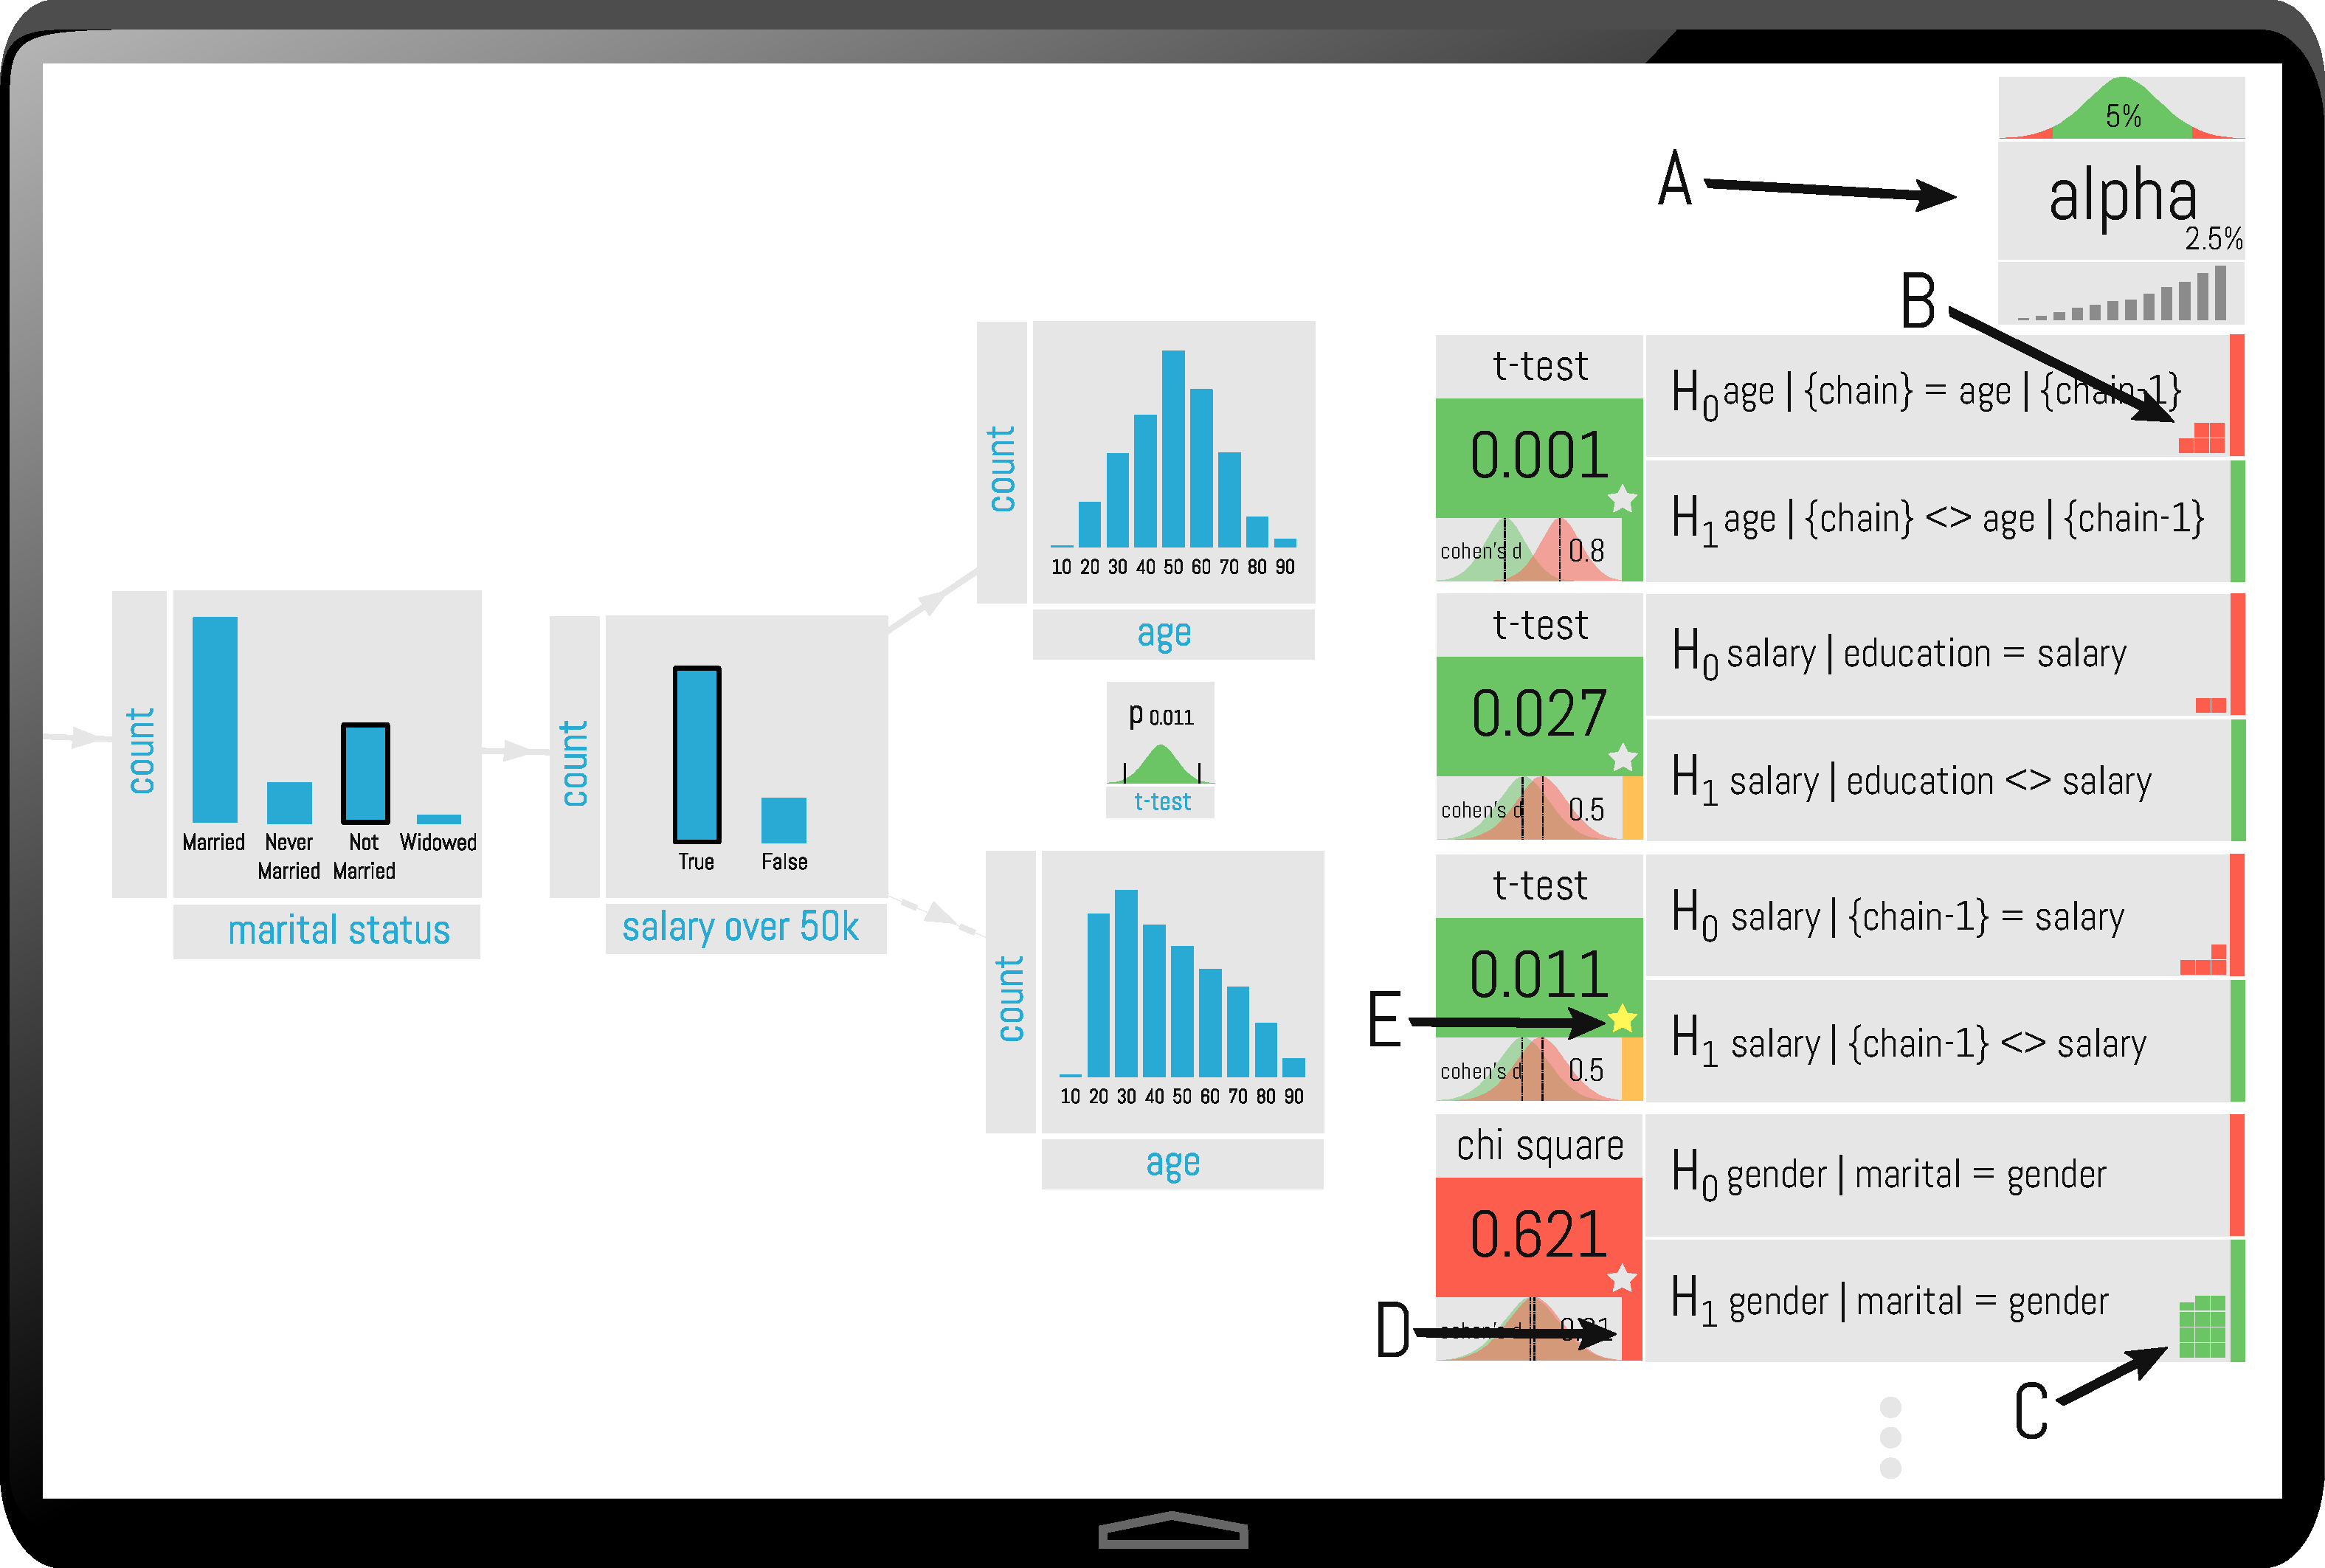
\includegraphics[width=0.48\textwidth]{figures/risk_controller}
\caption{The \system{} User Interface}
\label{fig:riskcontroller}	
\end{figure}

Figure \ref{fig:riskcontroller}	shows the current interface design of \system{} with a risk controller, which incorporates the above ideas, running on a tablet. 
The user interface features an unbounded 2D canvas where chains of visualizations (such as the one shown in Figure \ref{fig:sb}) can be laid out in a free form fashion. 
A ``risk-gauge'' on the right-hand side of the display (Figure \ref{fig:riskcontroller} (A)) serves two purposes: 
%\tim{maybe use a different color for A, B, C in the figure to better highlight them. First I thought A is part of the gauge}
it gives users a summary of the underlying procedure (e.g., the budget for the false discovery rate set to 5\% with current remaining wealth of 2.5\%; %distribution of the \pvals of all tests as 
both explained in the next two sections) and it provides access to a scrollable list of all the hypothesis tests (implicit and explicit) that have been execute so far. 
Each list entry displays details about one test and its results.
Textual labels describe the null- and alternative-hypothesis and color coded \pvals  indicate if the null-hypothesis was rejected or accepted (green for rejected, red for accepted).  
Furthermore, it visualizes the distribution of null-hypothesis and alternative hypothesis and shows its difference, included an indication of its color coded effect size (D). 
%\tim{emanuel, would be good to have a pointer in the figure}
Tap gestures on a specific item allow users to change things like the default hypothesis or the type of test.  
Additionally other information such as an estimation of the size of an additional data  $n^{H1}$ that could make the observation significant can be displayed in each item. 
In the example this information is encoded through a set of small squares (B, C) where each square indicates the amount of data that is in the corresponding distribution. In (B) the five red squares tells us that we need 5x the amount of data from the null-distribution to flip this test form rejected to accepted or conversely in (C) 11.5x the amount of data from the alternative-distribution to rejected this hypothesis. 
Finally, we allow to mark important hypotheses by tapping the ``star'' icons (E). 
%\tim{Again a pointer would be good. }



%\subsection{Overall Control}
%\label{sec:ui:overall}

%- FDR slider
%- Current Realization

%\subsection{The Default Hypothesis}
%\label{sec:ui:default}



%\subsection{Changing The Default Test}
%\label{sec:ui:change}


%\subsection{Additional Information}
%\label{sec:ui:additional}
%- How much more data we need to change the \pval
%- How much more data from the null-hypothesis do we need to add to flip it again

\subsection{Backend}
\label{sec:backend}
\sam{todo: describe system design choices, such as how to generate null hypotheses given user interactions, how to progressively compute marginalized false discovery rate in parallel, etc.}